%%%%%%%%%%%%%%%%%%%%%%%%%%%%%%%%%%%%%%%%%%%%%%%%%%%%%
%% File: main.tex
%% Authors: Petros Chanas, Konstantinos Vasilopoulos
%% Last update: April, 2022
%% Description: Provides our assignment 
%% regarding Open Source Software Quality Testing
%%and parameters of rating the performance and quality
%%of software developed of open source applications
%%%%%%%%%%%%%%%%%%%AUEB2021-2022%%%%%%%%%%%%%%%%%%%%%
%% Character encoding: UTF-8
%%%%%%%%%%%%%%%%%%%%%%%%%%%%%%%%%%%%%%%%%%%%%%%%%%%%%


\documentclass[a4paper, 11pt]{article}
\usepackage[margin=1in]{geometry}
% Set the font (output) encoding
\usepackage[LGR]{fontenc}
\usepackage{afterpage}
\usepackage{pdfpages}
% Greek-specific commands
\usepackage[greek]{babel}
\usepackage{graphicx}
\usepackage[T1]{fontenc}
\usepackage{tgtermes}
%\usepackage{background}
\graphicspath{ {./images/} }
%\thispagestyle{empty}
%\backgroundsetup{
%scale=1,
%angle=0,
%opacity=.1,  %% adjust
%contents={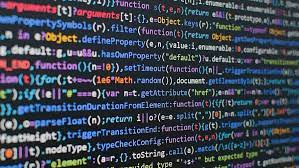
\includegraphics[width=\paperwidth,height=\paperheight]{images/sourceCode.jpg}}
%}
%
\includegraphics[width=\paperwidth, height=\paperwidth]{images/universe.jpg}}
\usepackage{hyperref}
\hypersetup{
    colorlinks=true,
    linkcolor=blue,
    filecolor=magenta,      
    urlcolor=blue,
    pdftitle={Overleaf Example},
    pdfpagemode=FullScreen,
    }

\urlstyle{same}

\title{\textbf{\textlatin{OPEN SOURCE SOFTWARE QUALITY}}}
\author{{\textit{Κωνσταντίνος Βασιλόπουλος\(\bullet\)3180018}\\*\textit{Πέτρος Χάνας\(\bullet\)3170173}}\\*
\includegraphics[width=4cm, height=3cm]{oSource}\\*
\fbox{Μπορείτε να βρείτε τον πηγαίο μας κώδικα \textlatin{Latex} στο \textlatin{\href{https://github.com/pkhaan/Open-Source-Software-Quality}{Github}}}}
\date{2022}

\begin{document}
\includepdf{assets/ekswfyllo.pdf}
\newpage
\thispagestyle{plain} % empty
\mbox{}
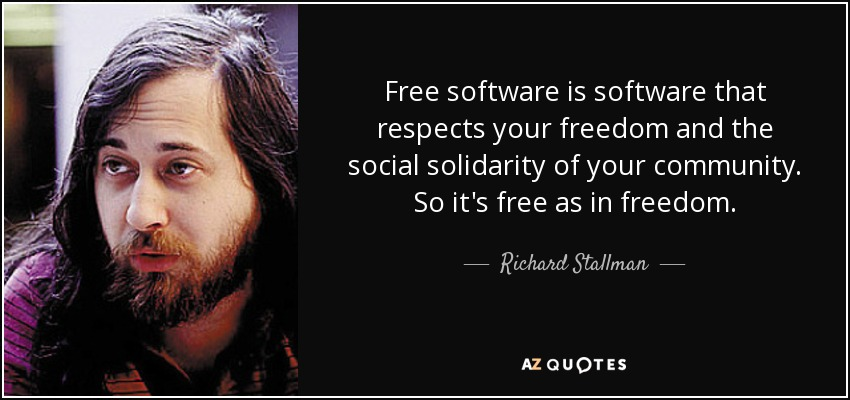
\includegraphics[width=15cm, height=8cm]{images/stallman.jpg}\\*
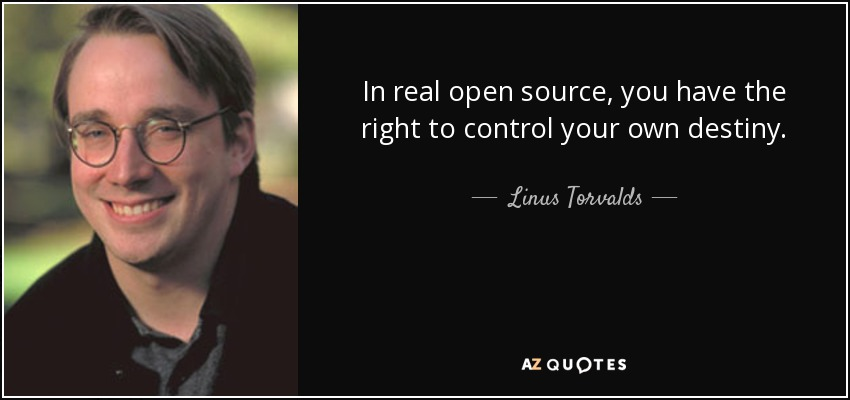
\includegraphics[width=15cm, height=8cm]{images/linus.jpg}\\*
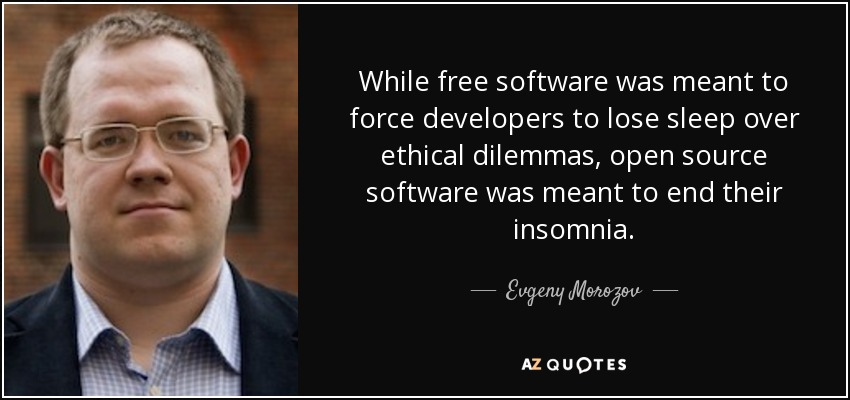
\includegraphics[width=15cm, height=8cm]{images/insomnia quote.jpg}
\maketitle

\tableofcontents


{\fontfamily{cmss}\selectfont

\begin{abstract}
Σε αυτήν την εργασία θα αναφερθούμε στους τρόπους ανάπυτηξης ελεύθερου λογισμικού
και στα ενδεχόμενα προβλήματα τα οποία προκύπτουν ως προς τον προγραμματισμό και το 
\textlatin{debugging} αυτού καθ'όλη τη διάρκεια ζωής του. Επίσης θα μελετήσουμε τους 
τρόπους αξιολόγησης του λογισμικού από τρίτους παράγοντες όπως εταιρείες, δημόσιοι οργανισμοί 
αλλά και από τους ίδιους τους χρήστες. Ουσιαστικα, η ποιότητα του ανοιχτού-ελεύθεροου λογισμικού 
συνίσταται από κάποιους βασικούς πυλώνες άμεσα εξαρτώμενος από το ίδιο το λογισμικό όπως η ταχύτητά
του, η αξιοπιστία του, η ευκολία στην χρήση του αλλά και την περιήγησή του και πολλά άλλα. Εν ολίγοις, 
θα αναλύσουμε όλες τις πτυχές ανάπτυξης και αξιολόγησης της ποιότητας λογισμικού ανοιχτού κώδικα 
διανθίζοντας όλα τα επιμέρους στοιχεία που συγκροτούν αλλά και καθιστούν το λογισμικό έτοιμο προς διάθεση 
στο ευρύ κοινό.
\end{abstract}

{\fontfamily{cmss}\selectfont\section{Τι είναι το λογισμικό ανοιχτού κώδικα\textlatin{;}}}
%%perigrafh open source code by definition
%%famous examples etc.
 Συχνά θα ακούσουμε ανθρώπους της πληροφορικής να αναφέρονται σε συγκεκριμένα προγράμματα ως «ανοιχτού κώδικα» ή «ελεύθερου λογισμικού». Εάν ένα πρόγραμμα είναι ανοιχτού κώδικα, ο πηγαίος κώδικας του είναι ελεύθερος διαθέσιμος στους χρήστες του. Οι χρήστες του - και οποιοσδήποτε άλλος - έχουν τη δυνατότητα να λάβουν αυτόν τον πηγαίο κώδικα, να τον τροποποιήσουν και να διανείμουν τις δικές τους εκδόσεις του προγράμματος. Οι χρήστες έχουν επίσης τη δυνατότητα να διανέμουν όσα αντίγραφα του αρχικού προγράμματος θέλουν. Οποιοσδήποτε μπορεί να χρησιμοποιήσει το πρόγραμμα για οποιονδήποτε σκοπό. δεν υπάρχουν χρεώσεις αδειοδότησης ή άλλοι περιορισμοί στο λογισμικό. Για παράδειγμα, το \textlatin{Ubuntu Linux} είναι ένα λειτουργικό σύστημα ανοιχτού κώδικα. Μπορείτε να κατεβάσετε το \textlatin{Ubuntu}, να δημιουργήσετε όσα αντίγραφα θέλετε και να τα δώσετε στους φίλους σας. Μπορείτε να εγκαταστήσετε το \textlatin{Ubuntu} σε απεριόριστο αριθμό υπολογιστών. Μπορείτε να δημιουργήσετε αντίγραφα του δίσκου εγκατάστασης του \textlatin{Ubuntu} και να τα διανείμετε. Εάν είχατε ιδιαίτερα κίνητρα, θα μπορούσατε να κατεβάσετε τον πηγαίο κώδικα για ένα πρόγραμμα στο \textlatin{Ubuntu} και να το τροποποιήσετε, δημιουργώντας τη δική σας προσαρμοσμένη έκδοση αυτού του προγράμματος - ή του ίδιου του \textlatin{Ubuntu}. Όλες οι άδειες ανοιχτού κώδικα σάς επιτρέπουν να το κάνετε αυτό, ενώ οι άδειες κλειστού κώδικα επιβάλλουν περιορισμούς σε εσάς.\\*
\\*
\section{Ιστορική Αναδρομή}
Κατά τη διάρκεια των πρώτων δεκαετιών της πληροφορικής, ήταν ο κανόνας και όχι η εξαίρεση η κοινή χρήση αναγνώσιμου πηγαίου κώδικα από τον άνθρωπο. Στις δεκαετίες του 1950 και του 1960 σχεδόν όλο το λογισμικό που παρήχθη από ακαδημαϊκούς και εταιρικά ερευνητικά εργαστήρια, όπως τα \textlatin{Bell Labs} της  \textlatin{AT&T}, εργάστηκαν σε συνεργασία. Όλοι είχαν μακροχρόνιες παραδόσεις ανοιχτού χαρακτήρα και συνεργασίας, άτυπες για τον ακαδημαϊκό χώρο, και ως εκ τούτου, ακόμη κι αν το λογισμικό δεν ήταν επίσημα διαθέσιμο στο κοινό, ο πηγαίος κώδικας τους ήταν ευρέως κοινός. Οι εταιρείες ηλεκτρονικών υπολογιστών διένειμαν επίσης τον πηγαίο κώδικα του λογισμικού που έστειλαν μαζί με το υλικό, για δύο λόγους. Πρώτον, δεν έβλεπαν το λογισμικό ως εμπόρευμα προς πώληση μέσω αδειοδότησης. Δεύτερον, οι χρήστες τροποποιούσαν συχνά οι ίδιοι το λογισμικό επειδή δεν θα λειτουργούσε σε διαφορετικό υλικό ή λειτουργικό σύστημα χωρίς κάποια παρέμβαση στον "κορμό" του, καθώς και για να διορθώσουν σφάλματα ή να προσθέσουν νέες λειτουργίες.

Το να έχουν διαθέσιμο τον πηγαίο κώδικα ήταν νευραλγικής σημασίας για τους κατασκευαστές, καθώς η δημιουργία διαφορετικών \textlatin{binary files} (ή μεταγλωττισμένου κώδικα) για διαφορετικό υλικό δεν ήταν καθόλου πρακτική και 
συχνά δημιουργούσε μεγάλες επιπλοκές που οδηγοούσαν σε λογισμικό μή προσπελάσιμο λογισμικό, δλδ μη ικανό να περαιωθούν οι λειτουργίες του. Ορισμένα πανεπιστήμια είχαν ακόμη και μια πολιτική που απαιτούσε όλα τα λογισμικά που είναι εγκατεστημένα στους υπολογιστές στα εργαστήριά τους να συνοδεύονται από δημοσιευμένους πηγαίους κώδικες.

Το 1953, το τμήμα \textlatin{UNIVAC} του \textlatin{Remington Rand} ανέπτυξε την πρώτη παρουσία ελεύθερου λογισμικού ανοιχτού κώδικα που ονομάζεται  \textlatin{A-2 (Arithmetic Language v2 system)}, το οποίο κυκλοφόρησε στους πελάτες τους μαζί με τον πηγαίο κώδικα. Προσκλήθηκαν επίσης να στείλουν πίσω τις βελτιώσεις τους. Αργότερα, το πρώτο λειτουργικό σύστημα της  \textlatin{IBM}, ο κώδικας του  \textlatin{IBM 704} διανεμήθηκε με όλους τους μεγάλους υπολογιστές τους. Οργανισμοί όπως η \textlatin{IBM}, η \textlatin{DEC} και η \textlatin{General Motors} δημιουργούν ομάδες χρηστών για να διευκολύνουν την κοινή χρήση κώδικα μεταξύ των χρηστών, ακαδημαϊκών και άλλων
παραγόντων του κλάδου. 

Με την πάροδο των δεκαετιών και την συνεχώς αναπτυσσόμενη βιομηχανία της τεχνολογίας ποικίλοι παράγοντες απαιτούσαν την διανομή, σε μεγαλύτερο βεληνεκές, ανοιχτού κώδικα λογισμικού για την κάλυψη των ήδη υπαρχουσών αναγκών. O ανοιχτός κώδικας απεδείχθη ως 
το κύριο πλεονέκτημα μικρών ομάδων προγραμματιστών για την ανάπτυξη μεγάλων και ευρέου βεληνεκούς, τρόπον τινά, εφαρμογών και λογισμικού. Χαρακτηριστικότερο ίσως παράδειγμα αυτής της αυτοδυναμίας ανάπτυξης αποτελεί ο \textlatin{Linus Torvalds} που 
στις αρχές της δεκαετίας του 1990 κατάφερε να προγραμματίσει έναν καινούριο \textlatin{kernel} βασισμένο εκ των προτέρων αλλά όχι εξ'ολοκλήρου στο λειτουργικό 
\textlatin{UNIX}. Έτσι, η κοινότητα του ελεύθερου λογισμικού έλαβε το πρώτο πλήρες δωρεάν λειτουργικό σύστημα με τον πυρήνα του \textlatin{Linus Torvalds} σε συνδυασμό με το λειτουργικό σύστημα \textlatin{GNU}. Το \textlatin{Debian}, που ιδρύθηκε από τον \textlatin{Ian Murdock} το 1993, δεσμεύτηκε στις αρχές \textlatin{GNU} και \textlatin{FSF} του ελεύθερου λογισμικού. Μεταγενέστερα παραδείγματα ελεύθερου λογισμικού αποτελούν οι διανομές ή \textlatin{distros} του \textlatin{Linux} και πληθώρα πακέτων και προγραμμάτων διαθέσιμα ενδολειτουργικά όπως π.χ. το \textlatin{inkcape}, το \textlatin{gcalculator}, τα \textlatin{KDE} πακέτα και πολλά άλλα.

\subsection{Τι είναι το  \textlatin{Linux}}
%%Description of OSI as the future of Systems Intercommunications.
%%Το μοντέλο διασύνδεσης ανοιχτών συστημάτων \textlatin{OSI} είναι ένα εννοιολογικό μοντέλο που δημιουργήθηκε από τον Διεθνή Οργανισμό Τυποποίησης που επιτρέπει σε διάφορα συστήματα επικοινωνίας να επικοινωνούν χρησιμοποιώντας τυπικά πρωτόκολλα. Σε απλά αγγλικά, το \textlatin{OSI}παρέχει ένα πρότυπο για διαφορετικά συστήματα υπολογιστών ώστε να μπορούν να επικοινωνούν μεταξύ τους.

%%Το μοντέλο \textlatin{OSI} μπορεί να θεωρηθεί ως μια καθολική γλώσσα για τη δικτύωση υπολογιστών. Βασίζεται στην ιδέα του διαχωρισμού ενός συστήματος επικοινωνίας σε επτά αφηρημένα επίπεδα, το καθένα στοιβαγμένο στο τελευταίο.

Το \textlatin{Linux} είναι μια από τις δημοφιλείς εκδόσεις του λειτουργικού συστήματος \textlatin{UNIX}. Είναι ανοιχτού κώδικα καθώς ο πηγαίος κώδικας του είναι δωρεάν διαθέσιμος. Το \textlatin{Linux} σχεδιάστηκε λαμβάνοντας υπόψη τη συμβατότητα \textlatin{UNIX}. Η λίστα λειτουργιών του είναι αρκετά παρόμοια με αυτή του \textlatin{UNIX}. Ακριβώς όπως τα \textlatin{Windows}, \textlatin{iOS} και \textlatin{Mac OS}, το \textlatin{Linux} είναι μια από τις πιο δημοφιλείς πλατφόρμες στον πλανήτη. Το \textlatin{Android}, τροφοδοτείται από το λειτουργικό σύστημα \textlatin{Linux} και σχεδόν καθ'ολολκληρίαν όλα τα λειτουργικά υπεύθυνα για την διαχείριση και την λειτουργία \textlatin{servers} δουλεύουν πάνω σε \textlatin{Linux}. 

Η υιοθέτηση του \textlatin{Linux} στην μαζική παραγωγή, αντί της πρότερης χρήσης αποκλειστικά και μόνο από ερασιτέχνες, άρχισε να απογειώνεται για πρώτη φορά στα μέσα της δεκαετίας του 1990 στην κοινότητα των υπερυπολογιστών, όπου οργανισμοί όπως η \textlatin{NASA} άρχισαν να αντικαθιστούν τις ολοένα και πιο ακριβές μηχανές τους με ομάδες φθηνών εμπορευματικών υπολογιστών με \textlatin{Linux}. Η εμπορική χρήση ξεκίνησε όταν η \textlatin{Dell} και η \textlatin{IBM}, ακολουθούμενη από τη \textlatin{Hewlett-Packard}, άρχισαν να προσφέρουν υποστήριξη \textlatin{Linux} για να ξεφύγουν από το μονοπώλιο της \textlatin{Microsoft} στην αγορά λειτουργικών συστημάτων επιτραπέζιων υπολογιστών.

Σήμερα, τα συστήματα \textlatin{Linux} χρησιμοποιούνται σε όλους τους υπολογιστές, από τα ενσωματωμένα συστήματα έως σχεδόν όλους τους υπερυπολογιστές, και έχουν εξασφαλίσει μια θέση σε εγκαταστάσεις διακομιστή όπως η δημοφιλής στοίβα εφαρμογών \textlatin{LAMP}. Η χρήση των διανομών \textlatin{Linux} σε οικιακούς και εταιρικούς επιτραπέζιους υπολογιστές έχει αυξηθεί. Οι διανομές \textlatin{Linux} έχουν γίνει επίσης δημοφιλείς στην αγορά netbook, με πολλές συσκευές να αποστέλλονται με προσαρμοσμένες διανομές \textlatin{Linux} εγκατεστημένες και η \textlatin{Google} να κυκλοφορεί το δικό της \textlatin{Chrome OS} σχεδιασμένο για \textlatin{netbook}. 


\subsubsection{\textlatin{Ubuntu}}
Ίσως η διασημότερη διανομή  \textlatin{(distro) Linux} μέχρι σήμερα με χιλιάδες εφαρμογές σε  \textlatin{desktop},  \textlatin{server} και ακόμη και  \textlatin{mobile} περιβάλλοντα. Ονομάστηκε έτσι από την διάλεκτο των  \textlatin{Xhosa} των  \textlatin{Nguni}, μίας φυλής στην Νότιο Αφρική. Κυριολεκτικά, σημαίνει ανθρωπότητα και θέλει να επιδείξει τον καθ'θπερβολή τον ΄πανανθρώπινο' χαρακτήρα και φιλοσοφία του λειτουργικού που είναι ελεύθερο και δωρεάν από όλους προς όλους. Έχοντας αυτό υπ'όψιν, το  \textlatin{Ubuntu} δεν αναπτύσσεται ούτε συντηρείται από την κοινότητα των χρηστών αλλά από την εταιρεία  \textlatin{Canonical} που αποτελούν και τους ιδρυτές του. Δεν μπορεί όμως να θεωρηθεί καθ'ολοκληρίαν  \textlatin{proprietary software} καθώς ο  \textlatin{Kernel} εξακολουθεί να είναι ο  \textlatin{Linux}. Δίχως αμφιβολία το  \textlatin{Ubuntu} είναι το διασημότερο  \textlatin{distro} χάρη στην ευκολία χρήσης του, την απλότητα της γραφικής του διεπαφής και τον άμεσο παραλληλισμό του με την αντίπερα όχθη των πλέον συνηθισμένων  \textlatin{Windows}.

\subsubsection{\textlatin{Debian}}
Το  \textlatin{Debian} αναπτύσσεται από εθελοντές από όλο τον κόσμο. Δεν είναι ένα  \textlatin{proprietary} λογισμικό, το οποίο υποστηρίζεται από εταιρείες όπως πολλές άλλες διανομές  \textlatin{Linux}. Εν τοις πράγμασι, κανένας δεν μπορεί να ισχυριστεί πως του 'ανήκει' το \textlatin{Debian} καθώς υπεύθυνη για την συντήρηση του και τις εκάστοτε αναβαμίσεις του είναι η κοινότητα χρηστών του. Αυτή η ουσιώδης διαφορά του από τα \textlatin{Ubuntu} το καθιστούν ως πυλώνα της κίνησης του Ελεύθερου Λογισμικού και ως ένα από τα διασημότερα και πιο εμπορικά \textlatin{Linux Distros}. Το \textlatin{Debian} ξεκίνησε τον Αύγουστο του 1993 από τον \textlatin{Ian Murdock}, τότε προπτυχιακό στο Πανεπιστήμιο \textlatin{Purdue} όπου και  χρηματοδοτήθηκε από το έργο \textlatin{GNU} του Ιδρύματος Ελεύθερου Λογισμικού, του οργανισμού που ξεκίνησε ως ιδέα του \textlatin{Richard Stallman} και σχετίζεται με τη Γενική Δημόσια Άδεια (\textlatin{GPL}).
\subsection{\textlatin{GPL}}
Η άδεια \textlatin{GPL} αναφέρεται στη Γενική Δημόσια Άδεια του \textlatin{GNU} που χρησιμοποιείται ευρέως για λογισμικό ανοιχτού κώδικα, που γράφτηκε για πρώτη φορά από τον \textlatin{Richard Stallman} το 1989. Οι προγραμματιστές και οι οργανισμοί τη χρησιμοποιούν για να εμποδίσουν το λογισμικό να γίνει ιδιόκτητο. Ενοποίησε παρόμοιες άδειες που ήταν διαθέσιμες εκείνη την εποχή, αλλά κατά κύριο λόγο αποτελεί υλοποίηση της φιλοσοφίας του Ιδρύματος Ελεύθερου Λογισμικού (\textlatin{FSF}) και της αντίληψης του \textlatin{Stallman} για το \textlatin{copyleft} για την ανάπτυξη και διανομή λογισμικού.

Με άδεια \textlatin{GPL} (ή απλώς \textlatin{GPL}), ένας συγκεκριμένος χρήστης μπορεί ελεύθερα να χρησιμοποιεί, να τροποποιεί ή να αναδιανέμει λογισμικό χωρίς περιορισμούς. Ένα δημοφιλές παράδειγμα λογισμικού που χρησιμοποιεί \textlatin{GPL} είναι το \textlatin{WordPress}, που σημαίνει ότι ο καθένας μπορεί να χρησιμοποιήσει, να τροποποιήσει ή να επεκτείνει τον πηγαίο κώδικα όπως επιθυμεί.

Η άδεια δίνει στους χρήστες την δικαιδοσία να εκτελέσουν τα κάτωθι:

\begin{itemize}
\item Μπορούν να κατεβάσουν και να εκτελέσουν το λογισμικό ελεύθερα
\item Μπορούν να αλλάξουν τον πηγαίο κώδικα του λογισμικού
\item Μπορούν να αναδιανείμουν αντίγραφα του λογισμικού αυτούσια ή ακόμα και να τα τροποποιήσουν και να τα διανείμουν εξυπηρετώντας καλύτερα μία ανάγκη του ενδεχομένως να έχει προκύψει
\end{itemize}

H oυσία αυτής της άδειας, και όλων των παρεμφερών, είναι να διασφαλίζουν κατά το μέγιστο δυνατό την ελεύθερη ανάπτυξη, συντήρηση και διανομή του λογισμικού ανοιχτού κώδικα.





\subsection{\textlatin{Mozilla Firefox}}
\indent Άλλο ένα σπουδαίο παράδειγμα λογισμικού ανοιχτού κώδικα είναι το πρόγραμμα περιήγησης διαδικτύου {\textlatin{Mozilla Firefox}. Ο \textlatin{Firefox} είναι ένα δωρεάν πρόγραμμα περιήγησης ιστού που κυκλοφόρησε για πρώτη φορά σε έκδοση beta στις 23 Σεπτεμβρίου 2002, ως "Πρόγραμμα περιήγησης \textlatin{Mozilla}, αν και εσωτερικά είχε την κωδική ονομασία \textlatin{"Phoenix"}. Ο \textlatin{Firefox} 1.0 κυκλοφόρησε επίσημα στις 9 Νοεμβρίου 2004. O σκελετός του φυλλομετρητή είναι ανοιχτού κώδικα και προσβάσιμος στο ευρύ κοινό.

Ο \textlatin{Firefox} έγινε δημοφιλής εναλλακτική του \textlatin{Microsoft Internet Explorer} 6.0 όταν οι χρήστες αναζήτησαν ένα πρόγραμμα περιήγησης που θα μπορούσε να τους προστατεύει καλύτερα από λογισμικό υποκλοπής \textlatin{spyware} και κακόβουλους ιστοτόπους. Από το 2017, είναι το τέταρτο πιο δημοφιλές πρόγραμμα περιήγησης μετά το \textlatin{Google Chrome}, το \textlatin{Apple Safari} και το \textlatin{UC Browser.}

To  \textlatin{Mozila} χρησιμοποιεί την  \textlatin{Gecko Rendering Engine} για να προβάλλει τους ιστοτόπους δημιουργώντας έτσι  \textlatin{Real-time} απεικόνιση των ιστοσελιδών χωρίς σχεδόν καθόλο  \textlatin{intermediate lag}. Το  \textlatin{Gecko} είναι επίσης μια μηχανή περιήγησης που αναπτύχθηκε από την  \textlatin{Mozilla} που συγκροτεί το  \textlatin{Firefox}, το  \textlatin{mail client Thunderbird} και πολλά άλλα  \textlatin{components}. Όπως σχεδόν όλα τα  \textlatin{projects} της  \textlatin{Mozilla} έτσι και το  \textlatin{Gegko} είναι και αυτό  \textlatin{open-source}.




\section{Ποιότητα Λογισμικού}
\subsection{Ορισμός}
Η ποιότητα λογισμικού είναι μια αφηρημένη έννοια που γίνεται αντιληπτή και ερμηνευόμενη διαφορετικά
με βάση τις προσωπικές απόψεις και τα ενδιαφέροντά του. Για να λυθεί αυτή η ασάφεια, το \textlatin{ISO/IEC9126} (Διεθνής Οργανισμός Τυποποίησης 2001) παρέχει ένα πλαίσιο για
την αξιολόγηση της ποιότητας του λογισμικού. Ορίζει έξι χαρακτηριστικά ποιότητας λογισμικού, συχνά
αναφέρονται ως ποιοτικά χαρακτηριστικά:
\begin{itemize}
\item \textbf{Λειτουργικότητα}: Εάν το λογισμικό εκτελεί τις απαραίτητες λειτουργίες.
\item \textbf{Αξιοπιστία}: Η ικανότητα του λογισμικού να παράγει επανειλημένα έγκυρα αποτελέσματα άνευ προβλημάτων.
\item \textbf{Χρηστικότητα}: Ο βαθμός ευκολίας του λογισμικού από το μέσο χρήστη.
\item \textbf{Αποτελεσματικό}: Κατά πόσο το επιθυμητό αποτέλεσμα επιτυγχάνεται μετά το πέρας της λειτουργίας του λογισμικού.
\item \textbf{Συντηρησιμότητα}: Η ευκολία με την οποία αναβαθμίζεται το λογισμικό στα πιο σύγχρονα πρότυπα.
\item \textbf{Φορητότητα}: Η δυνατότητα του λογισμικού να λειτουργεί σε πολλά και διαφορετικά λειτοργικά συστήματα.
\end{itemize}

\subsection{Tρόποι Ελέγχου Ποιότητας}%petros
%ιστορικη αναδρομη-αναφορά στον ελεγχο ποιότητας
Ο έλεγχος του λογισμικού περιστρέφεται πρακτικά γύρω από 2 θεμελιώδεις έννοιες-της επαλήθευσης και της επικύρωσης. Έτσι, γίνεται βέβαιο ότι το λογισμικό συναντά τις ανάγκες του εκάστοτε χρήστη δίχως παρεκκλίσεις από τις απαιτήσεις του. Οι 2 βασικές ερβτήσεις που τίθενται στον \textlatin{developer} είναι:
\begin{itemize}
\item Αναπτύσσω το σωστό προϊόν\textlatin{;}(Επαλήθευση)
\item Αναπτύσσω σωστά/ορθά το προϊόν\textlatin{;}(Επικύρωση)
\end{itemize}
H ουσία των 2 αυτών παραγώγων συναρτάται άμεσα με την ποιότητα της ανάπτυξης του λογισμικού και όχι μόνο. Αυτό συμβαίνει, διότι χρησιμοποιώντας αυτούς του 2 πυλώνες βεβαιώνω πως ο τρόπος ανάπτυξης του λογισμικού βρίσκεται σε παραλληλία με τις απαιτήσεις του χρήστη. Σε ιδεατό επίπεδο, οι μέθοδοι ελέγχου ποιότητας παράγουν ένα μαθηματικό μοντέλο που μας δίνει την 'ποιότητα' του λογισμικού που παρήχθη πάντα συναρτόμενη με τις απαιτήσεις του χρήστη/πελάτη και με τους διαθέσιμους πόρους. Ενίοτε, αυτό το πόρισμα δεν είναι πάντα τόσο ακριβές και σαφές και εν προκειμένω δίνεται μία πιο γενική παράθεση του προβλήματος όχι σε τόσο φορμαλιστικά πλαίσια. \\
Επι παραδείγματι, θα ασχοληθούμε με την έννοια του κόστους στον έλεγχο της ποιότητας του λογισμικού. Η έννοια αυτή αφορά ποικίλους τομέις της διαδικασίας ανάπτυξης του λογισμικού που αναλύονται στους επιμέρους παράγοντες:
\begin{itemize}
\item Kόστος Πρόληψης 
\item Κόστος Επιθεώρησης
\item Κόστος Αξιολόγησης
\item Κόστος Βλαβών
\end{itemize}
Αυτές οι 4 βασικές κατηγορίες κόστους συνιστούν σαν σύνολο την έννοια του 'κόστους' ανάπτυξης λογισμικού. Ο λόγος για τον οποίο αναφέρεται στον τρόπο ελέγχου ποιότητας δεν είναι παρα για να τεθεί η μεταβλητή 'κόστος΄ στην συνάρτηση 'ποιότητα'.
Είναι προφανές, πως όσο και αν θέλω να αυξήσω την ποιότητα του λογισμικού μου έαν τίθεται περιορισμός στο κόστος ανάπτυξης τότε η προαναφερθείσα ποιότητα θα λάβει ένα άνω όριο συναρτήσει του διαθέσιμου κεφαλαίου. Αξίζει να σταθούμε για λίγο στον τομέα των λαθων.


\subsection{Εργαλεία Ελέγχου Ποιότητας}
Σε αυτόν τον τομέα θα αναφερθούμε στα αυτοματοποιημένα εργαλεία που μας παράσχουν \textlatin{metrics} και ενδελεχείς αναλύσεις περί της γενικότερης 'ποιότητας΄ αλλά και τους επιμέρους παράγοντες που την συγκροτούν.

Μπορούμε να πλαισιώσουμε την γενικότερη έννοια της ποιότητας του λογισμικού ρωτώντας κάποιες απλές αλλά νευραλγικής σημασίας ερωτήσεις που ενοποιούν το πεδίο ποιότητα και το καθιστούν εύκολα κατηγοριοποιήσιμο.
\subsubsection{Χρήσιμες Μετρικές Ποιότητας Ελέγχου}
\textbf{Αξιοπιστία λογισμικού (\textlatin{software reliability}) είναι η πιθανότητα το πρόγραμμα να λειτουργεί ικανοποιητικά για μία δεδομένη χρονική περίοδο.} 
\[R = \frac{MXMB}{1 + MXMB}\]

Όπου \(ΜΧΜΒ\) είναι ο μέσος χρόνος μεταξύ βλαβών.\\*
\\*
\textbf{Διαθεσιμότητα λογισμικού (\textlatin{software availability}) είναι η πιθανότητα ένα πρόγραμμα να λειτουργεί επιτυχώς (ικανοποιητικά) σύμφωνα με τις απαιτήσεις λογισμικού σε μια δεδομένη χρονική στιγμή}
\[A = \frac{MXMB}{MXMB + ΜΧΕΣ} \]
Όπου \(ΜΧΕΣ\) μέσος χρόνος επιδιόρθωσης σφάλματος και ΜΧΜΒ μέσος χρόνος μεταξύ βλαβών.\\*
\\*
\subsubsection{Εκτίμηση Αριθμού Σφαλμάτων}
Εάν σε κάποιο λογισμικού διασπείρουμε εσκεμμένα S σφάλματα τότε μπορούμε να προβούμε σε εκτίμηση των πραγματικών σφαλμάτων παρατηρώντας το ποσοστό επιτυχίας στην επισήμανση των διεσπαρμένων σφαλμάτων.
\[Ν = \frac{Sn}{s}\]
Όπου:\\*
-\(S\)  σύνολο διεσπαρμένων σφαλμάτων\\*
-\(n\)  επισημανθέντα μη-διεσπαρμένα σφάλματα\\*
-\(s\)  επισημανθέντα διεσπαρμένα σφάλματα\\*
-\(N\) σύνολο πραγματικών μη-διεσπαρμένων σφαλμάτων\\*
\\*
\underline{Γράφημα συσχέτισης μεταξύ υπάρξης σφαλμάτων και του πλήθους των ήδη εντοπισμένων}\\*
\\*
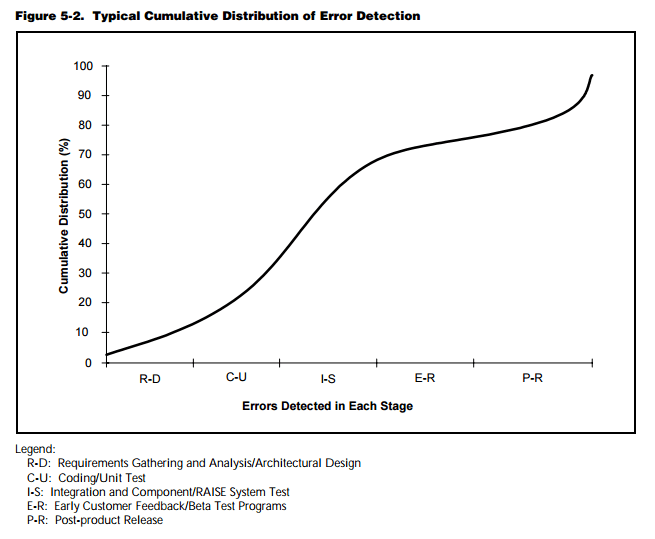
\includegraphics[width = 15cm, height = 12 cm]{images/errorGraph.png}\\*
\textit{Οι μετρικές που αναγράφονται εξηγούνται παρακάτω}\\*
\\*
\begin{itemize}
\item Εκτίμηση αριθμού σφαλμάτων με χρήση δύο διαφορετικών ομάδων ελέγχου.
\item Η αποτελεσματικότητα κάθε ομάδας ελέγχου μπορεί να μετρηθεί, υπολογίζοντας το κλάσμα των σφαλμάτων που βρέθηκαν από κάθε ομάδα.
\item Η αποτελεσματικότητα Ε(1) της ομάδας 1 μπορεί να εκφραστεί ως:  \(E(1) = x / n\)
\item Η αποτελεσματικότητα της ομάδας 2 ως \(E(2) = y / n\)
\item \(n = q / (E(1) × E(2))\), όπου \(q\) ο αριθμός των κοινών σφαλμάτων που βρήκαν οι ομάδες 1 και 2.
\end{itemize}
\\*
Έτσι, καταλήγουμε στην έννοια της \underline{εμπιστοσύνης} του λογισμικού όπου φορμαλιστικά είναι εν γένει η πιθανότητα να μην υπάρχει σφάλμα στο λογισμικό και δίνεται από τον παρακάτω τύπο \\*

\[C_n =
\left\{
	\begin{array}{ll}
		1  & \mbox{αν } n \geq N \\
		\frac{S}{S - N + 1} & \mbox{αν } n \leq N
	\end{array}
\right.\]
Ο παραπάνω τύπος εκφράζει την διασπρά σφαλμάτων και αναλύεται ως εξής:\\*
\begin{enumerate}
\item \(S\) αριθμός διεσπαρμένων σφαλμάτων
\item \(N\) αριθμός πραγματικών σφαλμάτων
\item \(n\) ο αριθμός των πραγματικών σφαλμάτων που επισημάνθηκαν
\end{enumerate}






\subsubsection{Μοντέλα Ποιότητας Ελέγχου}
\\*
\\*

Η σημασία της ποιότητας του λογισμικού εξακολουθεί να αποτελεί βασικό ενδιαφέρον για 
τις ακαδημαϊκές και βιομηχανικές κοινότητες μετά από περισσότερα από 50 χρόνια έρευνας. Επιπλέον, όπως ο αριθμός των πολύπλοκων δικτυωμένων συστημάτων και
οι υποδομές ζωτικής σημασίας που στηρίζονται σε αυτές αυξάνονται, αναμένεται να παραμείνει 
θέμα συνεχούς ενδιαφέροντος για έρευνα και συνεχή ανάπτυξη.
Προηγούμενη έρευνα για την ποιότητα του λογισμικού είχε ως αποτέλεσμα μεγάλο αριθμό ποιότητας
μοντέλα. Τα περισσότερα από αυτά περιγράφουν ένα σύνολο βασικών ιδιοτήτων που προσπαθούν να χαρακτηρίσουν τις πολλαπλές πτυχές ενός συστήματος λογισμικού από την πλευρά του πελάτη και από την πλευρά του προγραμματιστή αμφώτερα.
\\*



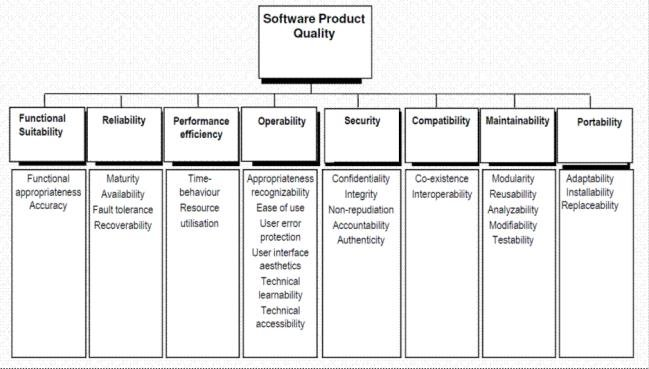
\includegraphics{images/ISO25010.jpg}\\*
\\*
\textbf{Παραπάνω παρουσιάζεται το ιεραρχικό μοντέλο: }
\textlatin{ISO25010}\\*

Η σημασία της ποιότητας του λογισμικού εξακολουθεί να αποτελεί βασικό ενδιαφέρον και για τα δύο
τις ακαδημαϊκές και βιομηχανικές κοινότητες μετά από περισσότερα από 50 χρόνια έρευνας
και πρακτική. Επιπλέον, όπως ο αριθμός των πολύπλοκων δικτυωμένων συστημάτων και
οι υποδομές ζωτικής σημασίας που στηρίζονται σε αυτές αυξάνονται, αναμένεται να παραμείνει α
θέμα συνεχούς ενδιαφέροντος για έρευνα, ανάπτυξη και συντήρηση λογισμικού.
Προηγούμενη έρευνα για την ποιότητα του λογισμικού είχε ως αποτέλεσμα μεγάλο αριθμό ποιότητας
μοντέλα. Τα περισσότερα από αυτά περιγράφουν ένα σύνολο βασικών ιδιοτήτων που προσπαθούν να το κάνουν
χαρακτηρίζουν τις πολλαπλές πτυχές ενός συστήματος λογισμικού από ένα εσωτερικό (προγραμματιστή-
προσανατολισμένη), εξωτερική (πελατοκεντρική) ή και των δύο προοπτικών.
Η εισαγωγή του πρώτου μοντέλου ποιότητας λογισμικού αποδίδεται στον \textlatin{McCall} in
1976, ακολουθούμενο από το μοντέλο \textlatin{Dromey} που το βελτίωσε. Αργότερα,
οι συνεισφορές έγιναν μέρος του προτύπου  \textlatin{ISO 9126}, το οποίο εξέφραζε λογισμικό
ποιότητας χρησιμοποιώντας ένα ιεραρχικό μοντέλο 5 τομέων ελέγχου που αποτελούνται από επιμέρους χαρακτηριστικά. Το μοντέλο  \textlatin{ISO 25010} που απεικονίζεται στο άνωθι σχήμα αντιπροσωπεύει την τρέχουσα έκδοση και θεωρεί τη δυνατότητα συντήρησης ως το σύνολο 5 βασικών
πυλώνων τροποποίησης: \\*
\begin{enumerate}
\item Αρθρωτότητα
\item Επαναχρησιμοποίηση
\item Αναλυσιμότητα
\item  Τροποποίηση
\item Δοκιμαστικότητα
\end{enumerate}
Η ουσία αυτών των χαρακτηριστικών δεν είναι απαραίτητα να βελτιώνουν τον κώδικα ενός προγράμματος ή μια δομής προγραμμάτων (λογισμικού) αλλά να παράσχουν σχολαστικές λεπτομέρειες σχετικά με την δυνατότητα της περαιτέρω ανάπτυξης αυτού.

Τα σημαντικά αποτελούμενα κομμάτια ενός λογισμικού εν γένει ονομάζονται \textlatin{metrics}.
Βασικές \textlatin{metrics} όπως γραμμές κώδικα, αριθμός συναρτήσεων ή αριθμός πακέτων και κλάσεων
οι ενότητες έχουν χρησιμοποιηθεί ευρέως και με τη σειρά τους, αντικαταστάθηκαν από την εισαγωγή του αντικειμενοστραφούς μοντέλου  και του σχετικού συνόλου μετρήσεων. Στις μέρες μας βρίσκουμε ένα
πλήθος αντικειμενοστρεφών \textlatin{metrics} όπως π.χ. αριθμός πακέτων και κλάσεων που ορίζονται και χρησιμοποιούνται για την ανίχνευση κομματιών κώδικα(προβληματικού),
ελαττωματικού σχεδιασμού ή για τη βελτίωση της συντηρησιμότητας. Αυτές οι μετρήσεις είναι επίσης
που απαιτούνται από τους ερευνητές για την αξιολόγηση της ποιότητας του λογισμικού σε ευρύτερο πλαίσιο. Ωστόσο, αυτό το μοντέλο φτάνει πια στην λήξη της λειτουργίας του στην αγορά και αντικαθίσταται πια από νέα που δίνουν έμφαση σε ποικίλους άλλους παράγοντες όπως η ταχύτητα του λογισμικού και η συμβασιμότητα αυτού με εργαλεία τεχνητης νοημοσύνης (ΑΙ) για την πιο υψηλού επιπέδου περάτωση και επίλυση ενός προβλήματος. 

\subsubsection{Δείκτης Πραγματικής Συντηρησιμότητας(\textlatin{Maintainability Index})}
Είχαν γίνει σημαντικές προσπάθειες για τη σωστή εκτίμηση των απαιτούμενων
πόρων για τη συντήρηση συστημάτων λογισμικού. Ορισμένος από τις αρχές της δεκαετίας του '70, η
υποθετική φόρμουλα για τον Δείκτη Συντηρησιμότητας (MI) ολοκληρώθηκε το 1992. Ο τύπος λαμβάνει υπόψη το μέγεθος του πηγαίου κώδικα, μετρούμενο συναρτήσει
    των παραλλαγών των γραμμών κώδικα και δύο παραμέτρους πολυπλοκότητας που εκφράζονται σε
όρους του αρθρωτού παραδείγματος. Το αρθρωτό παράδειγμα είναι ο αριθμός των λειτουργιών και των χρηστών, γνωστός και ως όγκος \textlatin{Halstead} που εκφράζει αριθμό των πιθανών διαδρομών και εναλλακτικών εκτέλεσης που δημιουργούνται από υπάρχουσες εντολές συνθηκών και βρόχους.
Ο τύπος εκφράζεται ώς:
\[M I = 171 − 5.2 ∗ ln(aveV ) − 0.23 ∗ aveG − 16.2 ∗ ln(aveST AT )\] όπου:  \(V\) απεικονίζει τον όγκο του \textlatin{Halstead}\\*
\(aveG\) ο αριθμός των πιθανών μονοπατιών εκτέλεσης\\*
\(aveSTAT\) ο μέσος όρος των δηλώσεων μεταβλητών\\*
\\*
\subsubsection{\textlatin{ARiSA Compendium Model}}\\*
Η Σύνοψη Προτύπων Ποιότητας Λογισμικού και Μετρικών1 δημιουργήθηκε από
\textlatin{ARiSA} και ερευνητές από το Πανεπιστήμιο \textlatin{Linnaeus}. Αποσκοπεί στη μελέτη της εκ νέου
σχέση μεταξύ χαρακτηριστικών ποιότητας λογισμικού και μετρικών τιμών λογισμικού.
Η \textlatin{Compendium} μοντελοποιεί την ποιότητα λογισμικού σύμφωνα με το \textlatin{ISO 9126}, μια παλαιότερη έκδοση στην οικογένεια \textlatin{ISO} για πρότυπα ποιότητας λογισμικού.
Όπως και το προηγούμενο έτσι και το εν λόγω μοντέλο αποτελείται από κάποια χαρακτηριστικά-πυλώνες που αναλύονται σε κάποια βασικά επιμέρους. Tα βασικά χαρακτηριστικά της \textlatin{Arisa} είναι τα κάτωθι:
\begin{itemize}
\item Αναλυσιμότητα
\item Μεταβλητότητα
\item Συμμόρφωση, 
\item Σταθερότητα 
\item Δοκιμαστικότητα
\end{itemize}

Συχνά, παρατηρούμε πως ειδικα στο λογισμικό του ανοιχτού κωδικα παρατηρούνται στο στάδιο της δόμησης κώδικα προτού καταλήξει αυτός στο αποθετήριο ενός συστήματος ελέγχου υπάρχουν σοβαρά σφάλματα στην δομή του κωδικα πράγμα που τον καθιστά πιο δυσανάγνωστο και μερικές φορές ακόμα πιο πολύπλοκο χρονικά και χωρικά αντίστοιχα. Χαρακτηριστικό ήταν το παράδειγμα που σε μια μεγάλη αναβάθμιση του \textlatin{Debian} στα πολύ πρώιμα βήματά του στα μέσα της δεκαετίας του '90 το περιβάλλον \textlatin{Desktop} που τότε χρησιμοποιούσε \textlatin{Xfce} κολλούσε συνεχώς και  παρουσίαζε σημαντικά προβλήματα στην διεπαφή του με το σύτημα αρχειοθέτησης του \textlatin{Kernel}. To πρόβλημα αρκετά αργότερα αποδείχθηκε ότι δεν ήταν σφάλμα του κωδικα συντακτικό ή λογικό αλλά υπέρογκο κομμάτι κώδικα που δεν μπορούσαν να διαχειριστούν πιο αδύναμοι υπολογιστές έτσι καθιστώντας το λειτουργικό σύστημα ακατάλληλο για τον σκοπό που είχε δημιουργηθεί. Έτσι, με ένα απλό μοντέλο εγκυρότητας και επαληθευσιμότητας ο κώδικας θα μπορούσε να έχει "ελαφρώσει" \textlatin{debloated} από αχρείαστα \textlatin{metrics} και συνθήκες που αποτελούσαν βάρος πολυπλοκότητας στην εκτέλεση του προγράμματος.

 Για κάθε
μετρική επιρροή, η \textlatin{compendium} περιγράφει λεπτομερώς την κατεύθυνση και την ισχύ του ως προς την ροή του κώδικα. Αυτά τα στατιστικά ονομάζονται \textlatin{chevrons} και χρησιμοποιούνται
να διευκρινίσουν εάν οι αυξημένες τιμές στην πολυπλοκότητα της περαίωσης για τη δεδομένη μέτρηση οδηγούν σε βελτίωση ή
υποβάθμιση της συντηρησιμότητας. Ο αριθμός των \textlatin{chevron} αντιπροσωπεύει τη δύναμη
αυτής της συσχέτισης, με δύο chevron να αντιπροσωπεύουν μια ισχυρότερη σχέση όσον αφορά την συντηρησιμότητα που στην περίπτωση του λογισμικού ανοιχτού κώδικα είναι ιδιαίτερα σημαντική για κάθε επόμενο \textlatin{update}. Πολλές φορές σε αποθετήρια ανοιχτού κώδικα υπάρχει ο κανόνας να εμφανίζεται η δομή του κώδικα αλλά και \textlatin{snippets} που προσδιορίζουν benchmarks-κλειδιά αλλά και ο τρόπος που αυτός ο κώδικας συντηρείται και αναπτύσσεται με την συνοδεία πάντα σχολίων και οδηγιών εξωτερικά. \\*
\\*



Παρακάτω παρουσιάζεται αναλυτικά ο πίνακας των επιρροών της συντηρησιμότητας στο μοντέλο ARISA Compendium\\*

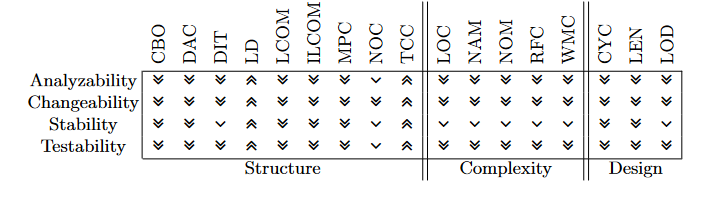
\includegraphics{images/arisa compendium.png}\\*
\\*
\begin{itemize}
\item \textlatin{CBO : coupling between objects}
\item \textlatin{DAC : data abstraction coupling}
\item \textlatin{DIT : depth of inheritance tree} 
\item \textlatin{LD  : Locality of data} 
\item \textlatin{LCOM : lack of cohesion in methods}
\item \textlatin{ILCOM : improved LCOM variant}
\item \textlatin{MPC : message pass coupling}
\item \textlatin{NOC : number of children} 
\item \textlatin{TCC : tight class cohesion}
\item \textlatin{LOC : Lines of code}
\item \textlatin{NAM : number of attributes and methods}
\item \textlatin{NOM : number of methods}
\item \textlatin{RFC : response for class}
\item \textlatin{WMC : weighted method count}
\item \textlatin{CYC : number of classes in cycle}
\item \textlatin{LEN : length of names}
\item \textlatin{LOD : Lack of Documentation}
\end{itemize}
\\*
Αυτά τα metrics αποτελούν την σύνθεση του μοντέλου έτσι ώστε να παραχθεί το απαιτούμενο αποτέλεσμα για την καταταξη της συντηρησιμότητας του λογισμικού.
\\*
Σε σύγκριση με το MI, το μοντέλο \textlatin{ARiSA} χρησιμοποιεί μια ευρύτερη επιλογή από 
μετρήσεις. Εκτός από τη μέτρηση \textlatin{LOC} που χρησιμοποιείται συνήθως, χρησιμοποιεί επίσης το WMC
ως μέτρηση πολυπλοκότητας, μαζί με πολλά γνωστά αντικειμενοστραφή μοντέλα ,
καλύπτοντας προβλήματα όπως η συνοχή, η σύζευξη και η κληρονομικότητα.
Ενώ ο MI μπορεί να υπολογιστεί σε διάφορα επίπεδα ευαισθησίας και ευπάθειας κώδικα,  το
μοντέλο \textlatin{ARiSA} περιορίζεται σε επίπεδο τάξης. Για να το κλιμακώσουμε σε επίπεδο συστήματος, εμείς
να υπολογίσουμε τη γεωμετρική του μέση τιμή σε όλες τις κατηγορίες συστημάτων.
\\*


\subsubsection{\textlatin{SQALE MODEL}}

To \textlatin{SQALE(Software Quality Assessment Based on Lifecycle Expectations)}
εισήχθη για πρώτη φορά από τον \textlatin{J.L. Letouzey} ως μέθοδος αξιολόγησης για 
την ποιότητα του πηγαίου κώδικα της εφαρμογής, με τρόπο ανεξάρτητο από τον γλώσσα προγραμματισμού
ή οποιοδήποτε άλλο εργαλείο ανάλυσης. Ίσως το πιο γνωστό τέτοιο εργαλείο είναι η πλατφόρμα κώδικα \textlatin{SonarQube}
που βασίζει την φιλοσοφία της στο μοντέλο \textlatin{SQALE}. To λογισμικό είναι ανοιχτού κώδικα και ελεύθερο προς χρήση.
Η υποστήριξη ανάλυσης παρέχεται μέσω plugins για συγκεκριμένη γλώσσα.
Υποστήριξη για πρόσθετες γλώσσες ή λειτουργίες
μπορεί να αναπτυχθεί με τη μορφή πρόσθετων plugins φτιαγμένων από εκάστοτε χρήστες. Για παράδειγμα, ο κώδικας \textlatin{C++} μπορεί να αναλυθεί
χρησιμοποιώντας μια δωρεάν προσθήκη που έχει αναπτυχθεί από την κοινότητα. Τα \textlatin{plugins} συνήθως περιλαμβάνουν έναν αριθμό από
κανόνες, έναντι των οποίων ελέγχεται το δέντρο αφηρημένης σύνταξης του πηγαίου κώδικα κατά τη διάρκεια
ανάλυσης. Ουσιαστικά, το λογισμικό διαθέτει μεθόδους που ελέγχουν snippets κώδικα του λογισμικού προς εξέταση ποιότητας και παράγουν μια εκτενή αναφορά με τυχόν ευπάθειες ή ευάλωτα σημεία στον κώδικα που δόθηκε. Κάθε κανόνας χαρακτηρίζεται από τη γλώσσα προγραμματισμού στην οποία εφαρμόζεται, τoν τύπο της
και τον τρόπο διερμηνείας της. Ο τύπος της κάθε γλώσσας είναι αυτός της  συντήρησης , αξιοπιστίας (πιθανότητα σφάλματος) ή ασφάλειας (τρωτότητα του προγράμματος). Το μοντέλο χρησιμοποιεί "ετικέτες" για να ταυτοποιήσει το εκάστοτε πρόβλημα
με κάθε ετικέτα να σχετίζεται με μία ή περισσότερες περιπτώσεις όπως
 αχρησιμοποίητος κώδικας, απόδοση ή υπερφόρτωση εγκεφάλου (π.χ. όταν η πολυπλοκότητα του κώδικα είναι πολύ υψηλή) ή ακόμα και λογικά λάθη στον κώδικα με την βοήθεια της τεχνητής νοημοσύνης σε πρόσφατα \textlatin{plugins}.
Η παραβίαση μιας ετικέτας οδηγεί σε ένα ζήτημα, το οποίο κληρονομεί τα χαρακτηριστικά του από την
ετικέτα που παραβιάστηκε. Για παράδειγμα, η ετικέτα \textlatin{Java S106} δηλώνει ότι "οι εκφράσεις
δεν πρέπει να είναι πολύ περίπλοκες».Η σωρεία ετικετών δημιουργεί κρίσιμα ζητήματα σοβαρότητας που επισημαίνονται
με υπερφόρτωση εγκεφάλου για εκφράσεις που περιλαμβάνουν περισσότερους από 3 τελεστές. Η ωρα
εκτιμάται ότι για να διορθωθεί το πρόβλημα είναι ένας σταθερός χρόνος 5 λεπτών στον οποίο προστίθεται 1 λεπτό
για κάθε πρόσθετο χειριστή πάνω από το όριο. Αυτό πρακτικά σημαίνει ότι έχω αθοιστική πολυπλοκότητα όχι μόνο στο debugging του 
κώδικα καθ'αυτού αλλά και στην ανάλυση της ποιότητας του λογισμικού μου ιδιαίτερα σε περιπτώσεις που έχω \textlatin{conflicts} ετικετών.
H συνολική τεχνική ωφέλεια μιας εφαρμογής υπολογίζεται ως το άθροισμα του εκτιμώμενου
χρόνου που απαιτείται για την επίλυση όλων των προβλημάτων που εντοπίστηκαν. Άρα, η έννοια της "τεχνικής ωφέλειας" είναι αυτή που εν τοιάυτη περιπτώσει συγκροτεί το μοντέλο και μαθηματικοποιεί τα παραγόμενα αποτελέσματά του.

Το \textlatin{SonarQube} χρησιμοποιεί τον ακόλουθο μαθηματικό τύπο για να παράξει μια ακόλουθη προσέγγιση της τεχνικής ωφέλειας του δοσμένου λογισμικού.
\\*
Η συνολική τεχνική ωφέλεια μίας εφαρμογής ή ενός λογισμικού συγκροτείται από τον ακόλουθο μαθηματικό τύπο:
\[T DR = \frac{TD}{DevT ime} \]

όπου \(TD\) η συνολική τεχνική ωφέλεια του προγράμματος εκφρασμένη σε λεπτά 
και \(DevTime\) ο συνολικός χρόνος που απαιτείται από τους προγραμματιστές έτσι ώστε να αναπτύξουν το λογισμικό.

Ενώ το \textlatin{SonarQube} και παρόμοια εργαλεία παρέχουν ποσοτικά μοντέλα λογισμικού
ποιότητα, η υπάρχουσα έρευνα επισήμανε επίσης ορισμένες υπάρχουσες παγίδες. Συγγραφείς κώδικα σε \textlatin{project} ανοιχτού κώδικα μεγάλης κλίμακας έδειξαν ότι πολλά από τα αναφερόμενα ζητήματα παρέμειναν
μη διορθωμένα το οποίο θα μπορούσε να είναι το αποτέλεσμα αυτών των εργαλείων που αναφέρουν πολλά ψευδώς θετικά αποτελέσματα,
ή αποτελέσματα χαμηλής σημασίας. Μια μελέτη των προεπιλεγμένων κανόνων του \textlatin{SonarQube} έδειξε επίσης
τα περισσότερα από αυτά έχουν περιορισμένη τάση σε σφάλματα. Αυτό σημαίνει ότι λογισμικά όπως το \textlatin{SonarQube} ή παρόμοια μπορούν να χρησιμοποιηθούν στην ανάπτυξη λογισμικού χωρίς όμως αυτό να προϋποθέτει πως δεν πρέπει να υπάρχουν συμπληρωματικά μοντέλα ελέγχου που προκαθορίζουν τα πλαίσια ανάπτυξης προς αποφυγή περαιτέρω σφαλμάτων.

\subsection{Απειλές στην Εγκυρότητα Λογισμικού}
Έτσι ώστε να διατηρείται η εγκυρότητα σε ένα κομμάτι λογισμικού οφείλουν να τηρούνται 3 βασικές αρχές
\begin{itemize}
\item Δομική Εγκυρότητα: Η απειλή στην δομική εγκυρότητα ενός προγράμματος απορρέει από εσφαλμένα βαθμονομημένες μετρικές κώδικα, δηλαδή από κακώς ορισμένα και αριθμημένα στοιχεία κώδικα που συντελούν σε διαρροή στον έλεγχο εγκυρότητας, π.χ. δεν λαμβάνονται υπ'όψιν οι ανάφορές \textlatin{@param} ως μετρική.
\item Εξωτερική Εκγυρότητα: Εδώ εστιάζουμε σε συγκεκριμένους εξωτερικούς παράγοντες δηλαδή εκτός περιβάλλοντος ανάπτυξης του λογισμικού όπως κάποια εσφαλμένη διαχείριση στους \textlatin{servers} που είναι υπεύθυνοι για την διαχείριση  \textlatin{storage} των δεδομένων του λογισμικού. Μπορούμε να ελαχιστοποιήσουμε αυτήν την άπειλη χρησιμοποιώτας τα πρωτόκολλα διαχείρισης του \textlatin{OSI: Open Source Initiative}
\item Εγκυρότητα συμπερασμάτων : Η απειλή  αφορά τα συμπεράσματα που έγιναν για την οικοδόμηση των μακροεντολών. Με ένα απλό παράδειγμα όταν πραγματοποιούμε έλεγχο με \textlatin{JUnit} και δεν αξιολογούμε διακριτά όλα τα επιμέρους κομμάτια του λογισμικού δημιοργείται σφάλμα μακροεντολής δηλαδή αδυναμία του λογισμικού να περαιώσει μια τάδε λειτουργία λόγω ενδεχόμενου λάθους σε αυτή. 
\end{itemize}

\subsection{Σύγχρονοι Μέθοδοι Ανάπτυξης Ανοιχτού Λογισμικού}

Προτού προχωρήσουμε στις σύχρονες μεθόδους ελέγχου της ποιότητας του ανοιχτού λογισμικού είναι απαραίτητο να γνωρίζουμε πως αναπτύσσεται το ανοιχτό λογισμικό, έτσι ώστε να διατυπωθεί μια πιο ολοκληρωμένη εικόνα της διαδικασίας.

Αρχικά, η σχεδίαση και η υλοποίηση λογισμικού ανοιχτού κώδικα διαφέρει σημαντικά από την παραδοσιακή μέθοδο ανάπτυξης λογισμικού. Η μεθοδολογία ανάπτυξης τέτοιου λογισμικού δεν είναι ξεκάθαρη και είναι δύσκολο να διαπιστωθούν τα μεμονωμένα τμήματα από τα οποία αποτελείται. Για αυτό το λόγο, \textlatin{project} ανοιχτού κώδικα έχουν δεχτεί σκληρή κριτική για την αδαφάνεια της διαδικασίας ανάπτυξης τους.

Αυτό είναι και το μαγαλύτερο εμπόδιο που πρέπει να υπερβεί κανείς καθώς εισέρχεται στον κόσμο της σχεδίασης ανοιχτού λογισμικού. Εφόσον δεν υπάρχει μία ξεκάθαρα δομημένη διαδικασία, την οποία ένας νέος προγραμματιστής μπορεί να ακολουθήσει, απαιτείται πειραματισμός και απόκτηση έμπρακτης εμπειρίας για να κατανοήσει κανείς τις διαδικασίες και τις φάσεις της ανάπτυξης του ανοιχτού λογισμικού.

\subsubsection{Διαδικασία Ανάπτυξης Λογισμικού Ανοιχτού Κώδικα}

Αυτή η ενότητα ασχολείται με τις σύγχρονες, τελευταίας γενιάς μεθόδους σχεδίασης και ανάπτυξης που αφορούν το λογισμικό ανοιχτού κώδικα(στο εξής \textlatin{OSS - Open Source Software}). Πιο συγκεκριμένα, αναφέρονται ονομαστικά τα βήματα που ακολουθάει ένας προγραμματιστής κατά την ανάπτυξη \textlatin{OSS}. Συνοπτικά, τα βήματα που ακολουθούνται έχουν εξής:

\begin{enumerate}
    \item Έρευνα απαιτήσεων
    \item Ανακάλυψη προβλήματος ή ένταξη νέας λειτουργίας
    \item Επιλογή η ανάθεση προβλήματος/λειτουργίας
    \item Αναζήτηση λύσης
    \item Ανάπτυξη κώδικα
    \item Προσθήκη κώδικα στο αποθετήριο
    \item Έλεγχος μονάδας
    \item Ανασκόπηση κώδικα
    \item Σύνταξη αναφοράς γνώμεων
    \item Περαιτέρω βήματα με σκοπό την προσθήκη του νέου κώδικα στην τελική έκδοση του λογισμικού
\end{enumerate}

Το τελευταίο βήμα, το οποίο αποσκοπεί στην ένταξη των αλλαγών στην τελευταία εκδοχή του κώδικα, είναι ουσιαστικά μία σειρά από βήματα τα οποία εξαρτόνται από το είδος του λογισμικού, το μέγεθος της ομάδας και την κατάσταση του \textlatin{project}. Για παράδειγμα, μια μικρή ομάδα ενδέχεται να μην συζητάει και να μην αναλύει κάθε μεμονωμένη προσθήκη κώδικα ή να μην διαθέτει το λογισμικό στους χρήστες σε \textlatin{pre-Alpha} έκδοση. Τέτοιοι παράγοντες επηρεάζουν τα τελευταία βήματα της ανάπτυξης και για αυτό δεν μπορούν να παρατεθούν τα τελικά βήματα εν συντομία, εντός της παραπάνω λίστας.

Επιπλέον, ορισμένες ομάδες προγραμματιστών έχουν επιλέξει μία πρακτική συνεχόμενης ενσωμάτωσης κώδικα (\textlatin{continuous integration practice}). Σύμφωνα με αυτή την πρακτική, νέος κώδικας ενσωματώνεται συνέχεια και με γρήγορους ρυθμούς στον κεντρικό σκελετό του λογισμικού. Αυτή η διαδικασία καθιστά αναγκαία την υιοθέτηση μεθόδων που επιτρέπουν την άμεση και άνευ καθυστερήσεων ανασκόπηση του νέου κώδικα. Αυτό που συνήθως υιοθετείται είναι αναφορές από τις γνώμες και τις απόψεις των μελών της υπόλοιπης ομάδας μέχρις ότου ο νέος κώδικας να τηρεί ορισμένα κριτήρια που θέτει η ομάδα.

\subsubsection{Χαρακτηριστικά Διαδικασίας Ανάπτυξης Λογισμικού Ανοιχτού Κώδικα}

Η ειδοποιός διαφορά ανάμεσα στην ανάπτυξη λογισμικού ανοιχτού κώδικα και στην ανάπτυξη του παραδοσιακού λογισμικού εντοπίζεται στο ότι οι προγραμματιστές \textlatin{OSS} δεν περνούν κάποια επίσημη διαδικασία προτού είναι σε θέση να προσφέρουν κώδικα. Οι προσθήκες κώδικα γίνονται κατά δύο τρόπους: την δημιουργία νέων χαρακτηριστικών και την διόρθωση λαθών(\textlatin{bugs}).

Τα νέα χαρακτηριστικά ορίζονται συνήθως από τους κύριους προγραμματιστές του \textlatin{OSS}, οι οποίοι ελέγχουν και την δομή του πρότζεκτ. Παρόλα αυτά, "μικρότεροι" προγραμματιστές ενδέχεται να δημιουργήσουν και αυτοί νέα χαρακτηριστικά ή να δημιουργήσουν ομάδες προγραμματιστών με σκοπό την δημιουργία ενός νέου \textlatin{feature}.

Αφού τα νέα, επιθυμητά χαρακτηριστικά οριστούν ή αφού ήδη υπάρχοντα προβλήματα εντοπιστούν δημιουργόυνται τα λεγόμενα \textlatin{issues}, συνήθως σε μια ιστοσελίδα όπως το \textlatin{Github} που φιλοξενεί τον κώδικα του \textlatin{OSS}, και μετέπειτα αναλαμβάνονται από προγραμαματιστές. Αυτή η ανάληψη εργασιών γίνεται από τον ίδιο τον προγραμματιστή χωρίς το \textlatin{issue} να αναθέτεται σε αυτών από κάποιον άλλο. Ακόμα, σε πολλές εφαρμογές υπάρχουν τμήματα κώδικα που "ανήκουν" σε ορισμένα άτομα. Αυτά τα άτομα διατηρούν και αναπτύσσουν αυτό το συγκεκριμένο τμήμα του \textlatin{project}. Αυτό δεν σημαίνει πως άλλοι προγρμαματιστές δεν μπορούν να συνεισφέρουν εξαιτίας κάποιας απαγόρευσης. Αντ' αυτού, υπάρχει σεβασμός προς αυτά τα μέλη της κοινότητας και για αυτό οι υπόλοιποι προγραμματιστές δεν ασχολόνται με τα δικά τους κομμάτια.

Έπειτα, έχοντας αναλάβει ένα συγκεκριμένο κομμάτι κώδικα(το \textlatin{issue} δηλαδή), ο προγραμματιστής αναζητά να βρει τον τρόπο υλοποίησης του νέου χαρακτηριστικού ή επίλυσης του \textlatin{bug}. Ουσιαστικά, το άτομο αναζητά πολλαπλές λύσεις και από αυτές επιλέγει συνήθως αυτή που προσωπικά θεωρεί ως καλύτερη έναντι των άλλων. Σε μερικές περιπτώσεις, όπου χρησιμοποιούνται προγράμματα επικοινωνίας ανάμεσα στους \textlatin{developers}, το εν λόγω άτομο μπορεί να προωθήσει τις λύσεις που έχει βρει σε άλλα μέλη της ομάδας προκειμένου να ζητήσει μία δεύτερη γνώμη.

Κατά αυτόν τον τρόπο φτάνει ο προγραμματιστής στο κομμάτι της υλοποίησης του νέου \textlatin{feature} ή της επίλυσης του προβλήματος. Σε αυτό το σημείο συγγράφεται ο νέος κώδικας που υλοποιεί το ζητούμενο αποτέλεσμα. Δεδομένου πως οι προγραμματιστές δουλέυουν εθελοντικά, είναι ασφαλές να υποθέσουμε πως οι περισσότεροι από αυτούς είναι και "παθιασμένοι" με αυτό που κάνουν. Για αυτό τον λόγο το λογισμικό ανοιχτού κώδικα παράγει και πιο ποιοτικό αποτέλεσμα από ότι το ιδιοταγές.

Ως επόμενο βήμα της διαδικασίας, ο νέος κώδικας προστίθεται στο αποθετήριο κώδικα. Κάθε \textlatin{project} έχει την δική του πολιτική για την προσθήκη νέου κώδικα. Κάποιες ομάδες αφήνουν μόνο πεπειραμένους προγρμματιστές να προσθέτουν νέο κώδικα στην βάση. Οι προσθήκες των υπόλοιπων προγρμματιστών ελέγχονται τακτικά από έμπιστα μέλη έως ότου αυτοί να θεωρηθούν έμπιστα μέλη της ομάδας, όπου και τους δίνεται το ελεύθερο να ανεβάζουν νέο κώδικα μέσω \textlatin{commits} κατά βούληση. Ακόμα, είναι αναγκαίο να τονίσουμε πως το άτομο που ανεβάζει τον νέο κώδικα δεν είναι απαραίτητα και ο συγγραφέας του. Ορισμένες ομάδες έχουν άτομα αποκλειστικά υπεύθυνα για τα \textlatin{commits} και άλλους που μόνο προγραμματίζουν.

Ο νεοσύστατος όμως κώδικας δεν μπορεί να ενταχθεί απλά στο κεντρικό κλαδί του αποθετηρίου. Αυτό, διότι ενδέχεται η προσθήκη του να προκαλεί σφάλματα σε άλλα τμήματα του λογισμικού. Σε αυτό το σημείο έρχονται και τα χαρακτηριστικά της συντηρησιμότητας και της αρθρωτότητας του κώδικα, τα οποία κρίνουν κατά πόσο νέος κώδικας θα επηρεάσει το υπόλοιπο λογισμικό στο σύνολο του. Εν πάση περιπτώση και ανεξαρτήτως του πόσο καλά τετμημένο είναι το πρότζεκτ ή πόσο καλά προσεγμένος είναι ο νέος κώδικας, η ομάδα οφείλει να ελέγξει την λειτουργικότητα του \textlatin{project} συνολικά, τρέχοντας \textlatin{test} κώδικα.

Η πιο συνηθισμένη μορφή τεστ είναι αυτή του ελέγχου μονάδας(\textlatin{unit testing}).

% Part 1 graph
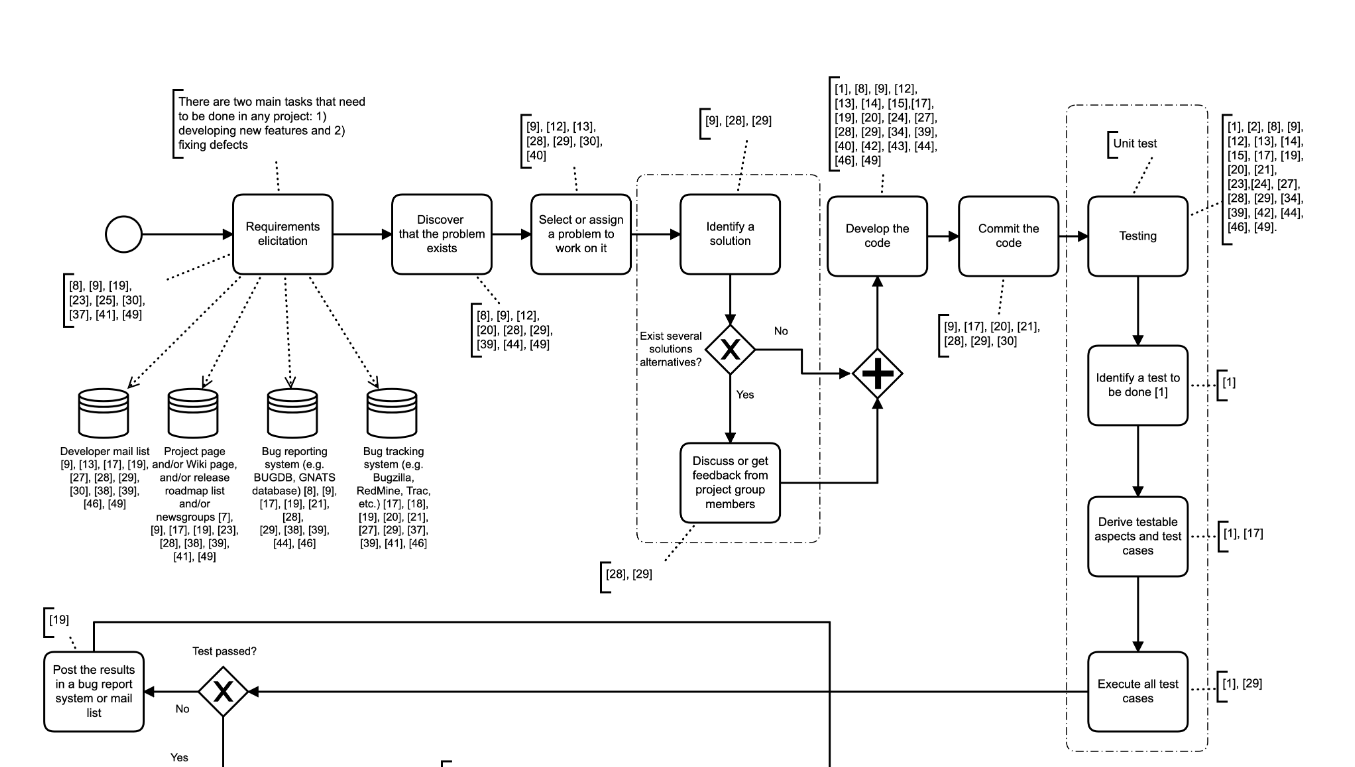
\includegraphics[
    width=\textwidth,
    height=\textheight,
    keepaspectratio
]{images/open_source_software_development_one.png}

% Part 2

% Part 2 graph
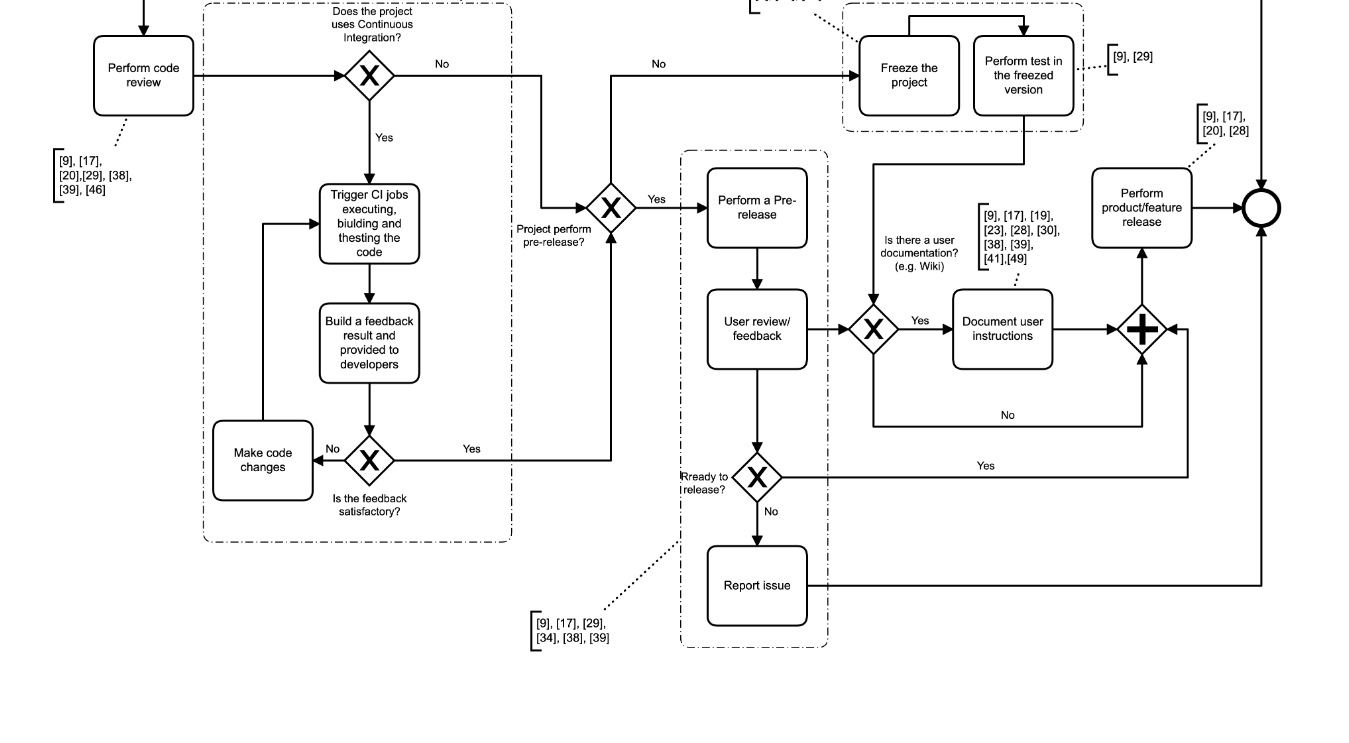
\includegraphics[
    width=\textwidth,
    height=\textheight,
    keepaspectratio
]{images/open_source_software_development_two.png}

% Epilogue

\subsection{Μοντέρνος Έλεγχος Ποιότητας}

Η παρακάτω ενότητα ασχολείται με τους σύγχρονους τρόπους ελέγχου της ποιότητας του λογισμικού. Ως επί το πλείστον, τα περισσότερα προγράμματα ανοιχτού κώδικα σχεδιάζονται και υλοποιούνται με την βοήθεια λογισμικού ελέγχου πηγαίου κώδικα(\textlatin{version control systems}), τα οποία επιτρέπουν σε μεγάλο αριθμό προγραμματιστών να συνεργάζονται πάνω στο ίδιο πρότζεκτ. Για αυτό το λόγο, η επόμενη υποενότητα αναλύει τα προγράμματα ελέγχου πηγαίου κώδικα.

\subsubsection{Λογισμικό Ελέγχου Πηγαίου Κώδικα}

Ο έλεγχος πηγαίου κώδικα ορίζεται ως η πρακτική σύμφωνα με την οποία παρακολουθούνται και διαχειρίζονται οι αλλαγές στον κώδικα του λογισμικού. Τα εργαλεία ελέγχου πηγαίου κώδικα είναι εξειδικευμένο λογισμικό, το οποίο συνεισφέρει στην διαχείριση του κώδικα από ομάδες προγραμματιστών. Ουσιαστικά, τα εν λόγω προγράμματα κρατούν κάθε αλλάγη στον πηγαίο κώδικα εντός μίας ειδικής βάσης δεδομένων. Εάν συμβεί κάποιο λάθος, οι προγραμματιστές μπορούν να επαναφέρουν τον πηγαίο κώδικα σε κάποια προηγούμενη έκδοση, αναιρώντας το πρόβλημα.

Επιπλέον, ο κώδικας ενός πρότζεκτ, μιας εφαρμογής ή ενός τμήματος λογισμικού είναι τυπικά οργανωμένος σε φακέλους. Έτσι, ένας προγραμματιστής μπορεί να δουλεύει ένα κομμάτι του κώδικας καθώς κάποιος άλλος αφαιρεί ένα \textlatin{bug} από ένα άλλο κομμάτι. Τα προγράμματα ελέγχου πηγαίου κώδικα συνεισφέρουν σε αυτή την διαδικασία καθώς καταγράφουν κάθε μεμονομένη αλλάγή από κάθε προγραμματιστή ξεχωριστά. Αλλαγές σε ένα κομμάτι του κώδικα ενδέχεται να μην είναι συμβατές με αυτές σε ένα άλλο τμήμα. Τέτοια προβλήματα πρέπει να αναγνωριστούν και να απομονωθούν δίχως να παρεμποδίζουν την ανάπτυξη του υπόλοιπου λογισμικού. Τα προγράμματα ελέγχου πηγαίου κώδικα μπορούν να διατηρούν πολλά κλαδιά(\textlatin{branches}) με διαφορετικές εκδόσεις του λογισμικού σε κάθε κλαδί, επιτρέποντας έτσι την εύκολη αντιμετώπιση των παραπάνω προβλημάτων.

Μακράν το πιο γνωστό λογισμικό ελέγχου πηγαίου κώδικα είναι το \textlatin{Git}. Το \textlatin{Git} είναι πλέον ενσωματωμένο σε πολλές πλατφόρμες και μπορεί να χρησιμοποιηθεί με πολλούς τρόπους. Γνωστά \textlatin{IDE} όπως το \textlatin{Visual Studio} της \textlatin{Microsoft}, το \textlatin{Android Studio} της \textlatin{Google} και πολλά άλλα, περιέχουν προεγκατεστημένο το \textlatin{Git} για πιο γρήγορο \textlatin{version control}. Υπάρχει φυσικά και η παραδοσιακή μέθοδος μέσω του \textlatin{terminal} ή και η επιλογή μίας γραφικής διεπαφής. Ακόμα, παρέχονται και διαδικτυές υπηρεσίες, όπως το \textlatin{Github}, το \textlatin{Gitlab} και το \textlatin{Bitbucket} που προσφέρουν γενικευμένες λύσεις στον τομέα του ελέγχου πηγαίου κώδικα. Άλλα λογισμικά ελέγχου πηγαίου κώδικα είναι το \textlatin{Mercurial} και το \textlatin{CVS(Concurrent Versions System)}.

\subsubsection{Αποφυγή Κακόβουλου Λογισμικού}

Το κύριο πρόβλημα ασφαλείας που αντιμετωπίζουν οι ομάδες ανάπτυξης ελεύθερου λογισμικού προκύπτει από το ότι ο καθένας είναι ελεύθερος να προσθέσει κώδικα στο \textlatin{project}. Κάποιος κακόβουλος προγραμματιστής θα μπορούσε να εισάγει λογισμικό το οποίο βλάπτει το πρόγραμμα ή τον χρήστη του. Για αυτό το λόγο, οι ομάδες που αναπτύσσουν τέτοιου είδους λογισμικό, σχεδόν πάντα, δεν επιτρέπουν την ενσωμάτωσει νέου κώδικα άνευ ελέγχου από κάποιο έμπειρο και έμπιστο μέλος της ομάδας. Ακόμα, ο νέος κώδικας συνηθίζεται να προστίθεται σε ξεχωριστά από το κεντρικό κλαδία του λογισμικού ελέγχου πηγαίου κώδικα. Έτσι, πριν την συγχώνευση των κλαδιών στο κεντρικό τμήμα, ο κώδικας επανελέγχεται για τυχόν επικίνδυνα κομμάτια κώδικα που διέφυγαν.

Ως αποτέλεσμα, ο λόγος για τον οποίο το λογισμικό ανοιχτού κώδικα θεωρείται και ασφαλείες είναι η ύπαρξη αυτής της "ομάδας ματιών" που συνεχώς κοιτάει τις νέες προσθήκες. Κάτι τέτοιο μπορεί να επιτευχθεί μόνο σε λογισμικό το οποίο είναι και διαθέσιμο άνευ πληρωμής, καθώς έτσι μπορεί να προσελκύσει μεγαλύτερο πλήθως ενδιαφερομένων.

Παρόλα αυτά, πρέπει να σημειωθεί πως τα περισσότερα πρότζεκτ τα διαχειρίζονται μικρές, ολιγομελείς ομάδες. Έτσι, δεν είναι ιδιαίτερα απίθανη η διείσδυση κακόβουλου κώδικα στο λογισμικό, καθώς και ο αριθμός των ατόμων που τακτικά επιθεωρούν τις νέες προσθήκες είναι μικρότερος. Επιπλέον, εκ φύσεως το ανοιχτό λογισμικό δεν αναγκάζει τους συνδρομητές ενός \textlatin{project} να το συντηρήσουν. Οπότε, η δυνατότητα συντήρησης ενός πρότζεκτ μειώνεται καθώς οι προγραμματιστές που συνέσφεραν κώδικα φεύγουν και νέοι προγραμματιστές δεν είναι διατεθιμένοι να ανατρέξουν στον παλαιό κώδικα για να τον ανανεώσουν. Αυτό σημαίνει πως νέες αδυναμίες που ανακαλύπτονται με την πάροδο του χρόνου δεν διορθώνονται και το λογισμικό παραμένει επιρρεπής σε γνωστές πλέον επιθέσεις.

Κατά αυτό τον τρόπο έχουν υπάρξει ορισμένες περιπτώσεις όπου λογισμικό ανοιχτού κώδικα παρέμενε ευάλωτο σε επιθέσεις για πολλά χρόνια χωρίς αυτό να ήταν γνωστό στην ομάδα που το διαχειρίζοταν. Για παράδειγμα, στις 13
Μαΐου του 2008 ανακαλύφθηκε πως η έκδοση \textlatin{Debian} του λειτουργικού συστήματος \textlatin{Linux} διέθεται μία γεννήτρια τυχαίων αριθμών, της οποίας η συμπεριφορά μπορούσε να προβλεθεί. Αυτό έμπρακτα σήμαινε, πως χιλίαδες πακέτα είχα κρυπτογραφηθεί κατά τρόπο προβλέψιμο και έτσι η ακεραιότητα των εν λόγω πακέτων τέθηκε υπό αμφισβήτηση.

Άλλη μία γνωστή περίπτωση, όπου λογισμικού ανοιχτού κώδικα χτυπήθηκε και παρέμεινε μολυσμένο για μεγάλο χρονικό διάστημα είναι αυτή του \textlatin{Webmin}. Το \textlatin{Webmin} είναι λογισμικό διαχείρισης και ελέγχου διακομιστών τύπου \textlatin{Unix}. Ένας άγνωστος \textlatin{hacker} κατάφερε να εμφυτέψει ένα πρόγραμμα απομακρυσμένης πρόσβασης (\textlatin{backdoor}) εντός της επίσημης έκδοδης του \textlatin{Webmin}. Ως αποτέλεσμα, ο κακόβουλος χρήστης μπορούσε να αποκτήσει πρόσβαση σε κάθε υπολογιστή που κατέβαζε και εγκαταστούσε το \textlatin{Webmin}. Αργότερα, αναγνωρίστηκε από την ομάδα σύνταξης του προγράμματος πως η συγκεκριμένη αδυναμία είχε παραμείνει κρυμμένη για περισσότερο από ένα χρόνο.

\textbf{\section{Ένα Αναλυτικό Παράδειγμα}}
\subsection{Λόγοι και Αφορμές}
\begin{itemize}
\item \textbf{Συνεργασία} Τα έργα ανοιχτού κώδικα μπορούν να δεχτούν αλλαγές από οποιονδήποτε στον κόσμο. Το \textlatin{Exercism}, για παράδειγμα, είναι μια πλατφόρμα ασκήσεων προγραμματισμού με περισσότερους από 350 συντελεστές.
\item \textbf{Υιοθέτηση και ανάμιξη}: Τα έργα ανοιχτού κώδικα μπορούν να χρησιμοποιηθούν από οποιονδήποτε για σχεδόν οποιονδήποτε σκοπό. Οι άνθρωποι μπορούν ακόμη και να το χρησιμοποιήσουν για να χτίσουν άλλα λογισμικά. Το \textlatin{WordPress}, για παράδειγμα, ξεκίνησε ως διχάλα ενός υπάρχοντος έργου που ονομάζεται \textlatin{b2}.
\item \textbf{Διαφάνεια}: Οποιοσδήποτε μπορεί να επιθεωρήσει ένα έργο ανοιχτού κώδικα για σφάλματα ή ασυνέπειες. Η διαφάνεια έχει σημασία για κυβερνήσεις όπως η Γερμανια ή οι Ηνωμένες Πολιτείες, για τις ανάλογες βιομηχανίες και υπηρεσίες όπως ο τραπεζικός τομέας και η υγειονομική περίθαλψη.
\end{itemize}

\subsection{Αρχίζοντας το \textlatin{project} ή μία συνεισφορά}
Για να μπορέσουμε να συμβάλλουμε σε ένα project ανοιχτού κώδικα πρέπει να ακολουθήσουμε κάποιους βασικούς κανόνες που επιβάλλει η κοινότητα όσον αφορά την κύρια ροή στα \textlatin{requests} των υποψήφιων \textlatin{developers}. Ο έλεγχος ποιότητας μπορεί να πραγματοποιηθεί και από εμάς αλλά τον τελευταίο λόγο θα τον έχει η ομάδα των \textlatin{moderators} του λογισμικού.

Πριν κάνoυμε οτιδήποτε, κάνουμε έναν γρήγορο έλεγχο για να βεβαιωθούμε ότι η ιδέα μας δεν έχει συζητηθεί αλλού. Παρακάμπτουμε το \textlatin{README} του έργου, τα \textlatin{requests (open και closed)}, και τη λίστα των \textlatin{logs}. Δεν χρειάζεται να ξοδεύoυμε ώρες εξετάζοντας τα πάντα, αλλά μια γρήγορη αναζήτηση για μερικούς βασικούς όρους είναι πολύ σημαντική.

Εάν δεν μπορούμε να βρούμε την ιδέα μας αλλού, είμαστε έτοιμοι να κάνουμε μια κίνηση. Εάν το έργο βρίσκεται στο \textlatin{GitHub}, πιθανότατα θα επικοινωνήσουμε με την ομάδα των προγραμματιστών  ανοίγοντας ένα issue ή ένα pull request.

    Τα issues είναι σαν να ξεκινάς μια συζήτηση όπου
    τα \textlatin{pull requests}  αφορούν την έναρξη εργασιών για μια λύση
    Για χαλαρή επικοινωνία, όπως διευκρινιστική ερώτηση, χρησιμοποιούμε  \textlatin{Stack Overflow, IRC, Slack ή άλλα κανάλια συνομιλίας}.

Προτού ανίξουμε ένα \textlatin{issue} ή \textlatin{pull request}, ελέγχουμε τα συνεισφέροντα έγγραφα του έργου (συνήθως ένα αρχείο που ονομάζεται \textlatin{CONTRIBUTING} ή στο \textlatin{README}), για να δούμε εάν χρειάζεται να συμπεριλάβουμε κάτι συγκεκριμένο. Για παράδειγμα, μπορεί να μας ζητηθεί να ακολουθήσουμε ένα πρότυπο ή να απαιτηθεί η χρήση δοκιμών.

\subsection{Συμβατικός Έλεγχος}
Προφανώς, προτού παραδόσουμε ένα λογισμικό προς χρήση οφείλουμε να προβούμε σε κάποιους ελέγχους που θα καθορίσουν την ποσόστωση της λειτουργικότητας του και το άν θα γίνει \textlatin{public} η όχι. Στην περίπτωση του ανοιχτού κώδικα ισχύουν ακριβώς οι ίδιοι παράγοντες με τα ιδιοταγή λογισμικά.\\*

Υπάρχουν τα κάτωθι στάδια ελέγχου:
\begin{itemize}
\item Ο έλεγχος λογισμικού έχει μία ροή από το «μικρό» (έλεγχος
μονάδας) προς το «μεγάλο» (έλεγχος συστήματος)
\item Έλεγχος μονάδας (\textlatin{unit testing}). Ο έλεγχος μίας μονάδας
λογισμικού (μία μέθοδος ή μία κλάση).
\end{itemize}
\\*
Στην παρακάτω εικόνα αναφέρεται σε αντίστοιχο σχεδιάγραμμα τα βήματα των σταδίων ελέγχου\\*
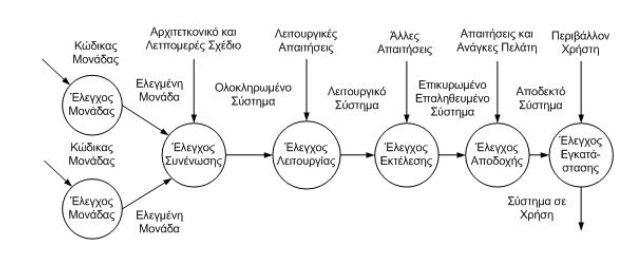
\includegraphics{images/control.png}\\*
\subsubsection{Έλεγχος μονάδας}
Η δοκιμή μονάδας είναι η διαδικασία συγγραφής και αυτόματης εκτέλεσης δοκιμών για να διασφαλιστεί ότι οι συναρτήσεις που κωδικοποιείτε λειτουργούν όπως αναμένεται. Παρόλο που μπορεί να φαίνεται σαν περισσότερη δουλειά, στην πραγματικότητα πρόκειται για τη λήψη προληπτικών μέτρων για την εξάλειψη των σφαλμάτων πριν αυτά εμφανιστούν.\\*

\begin{itemize}
\item Οι έλεγχοι μονάδας πραγματοποιούνται συνήθως από τους
προγραμματιστές και εστιάζουν στον έλεγχο της ορθότητας του
λογισμικού.
\item Συνήθως είναι έλεγχοι ανοιχτού κουτιού (white box testing) επειδή
ο έλεγχος γίνεται έχοντας γνώση της εσωτερικής δομής των
μονάδων που ελέγχονται.
\item Μπορεί όμως να είναι και έλεγχοι κλειστού κουτιού (black box)
χωρίς δηλαδή να λαμβάνουμε υπόψη την εσωτερική δομή των
μονάδων λογισμικού.
\end{itemize}

\subsection{Γενικότεροι Έλεγχοι}
Η σωστή εκσφαλμάτωση του λογισμικού πραγματοποιείται ανά στάδια και αποτελεί διαδικασία ενός συνόλου ελέγχων που συγκροτούν τον έλεγχο του συστήματος
\subsubsection{Έλεγχος Λειτουργίας}
Ο έλεγχος λειτουργίας εστιάζει στην ορθή λειτουργικότητα και
μπορεί να αυτοματοποιηθεί με κατάλληλα εργαλεία (π.χ. \textlatin{Selenium}).
\subsubsection{Έλεγχος Εκτέλεσης}
\begin{itemize}
\item Έλεγχοι πίεσης (\textlatin{(stress tests)}. Aξιολογούν το σύστημα όταν δουλεύει υπό πίεση, στα όρια του, σε μια σύντομη χρονική περίοδο.
\item Έλεγχοι χωρητικότητας \textlatin{(volume tests)}.  Δείχνουν πως το σύστημα χειρίζεται μεγάλες ποσότητες δεδομένων.
\item Έλεγχοι διάταξης \textlatin{(configuration tests)}. Αναλύουν τις διάφορες διατάξεις λογισμικού και υλικού που προσδιορίστηκαν από τις απαιτήσεις.
\item Έλεγχοι συμβατότητας \textlatin{(compatibility tests)}. Εξετάζεται αν οι λειτουργίες των διεπαφών εκτελούνται σύμφωνα με τις απαιτήσεις. 
\item Έλεγχοι παλινδρόμησης \textlatin{(regression tests)}. Οι έλεγχοι παλινδρόμησης εγγυώνται ότι η εκτέλεση του νέου συστήματος είναι τουλάχιστον τόσο καλή όσο και του παλαιού
\item Έλεγχοι ασφάλειας \textlatin{(security tests)}.  Διαβεβαιώνουν ότι οι απαιτήσεις ασφάλειας έχουν ικανοποιηθεί.
\item Έλεγχοι χρονισμού \textlatin{(timing tests)}.  Αποτιμούν τις απαιτήσεις που ασχολούνται με χρόνους απόκρισης και χρόνους εκτέλεσης μιας λειτουργίας
\item Περιβαλλοντικοί έλεγχοι \textlatin{(environmental tests)}. Εξετάζουν την ικανότητα του συστήματος να λειτουργεί στο χώρο εγκατάστασης. 
\item Έλεγχοι ποιότητας \textlatin{(quality tests)}. Αποτιμούν τα ποιοτικά χαρακτηριστικά του λογισμικού.
\item Έλεγχοι ανάκαμψης \textlatin{(recovery tests)}. Ασχολούνται με την απόκριση του συστήματος όταν υπάρχουν σφάλματα ή όταν χαθούν δεδομένα ή όταν δεν λειτουργούν συσκευές ή όταν πέσει η ισχύς. 
\item Έλεγχοι συντήρησης \textlatin{(maintenance tests)}. Επαληθεύουμε την ύπαρξη και σωστή λειτουργία αυτών των βοηθητικών μέσων συντήρησης.
\item Έλεγχοι τεκμηρίωσης \textlatin{(documentation tests)}. Επιβεβαιώνουν ότι έχουν γραφτεί τα απαιτούμενα έγγραφα τεκμηρίωσης.
\item Έλεγχοι ανθρώπινων παραγόντων \textlatin{(human factors tests)}. Ερευνούν τις απαιτήσεις που σχετίζονται με την διεπαφή του χρήστη με το σύστημα
\end{itemize}

\subsubsection{Έλεγχος Αποδοχής}
\begin{itemize}
\item \textlatin{benchmark test}: O έλεγχος που σχετίζεται με την δοκιμασία του δοθέντος λογισμικού στις περιπτώσεις εξαίρεσης της πλαισιωμένης λειτουργίας του και στην διαχείριση των σφαλμάτων του.
\item πιλοτικός έλεγχος (\textlatin{pilot test})
\item \textlatin{alpha test}
\item \textlatin{beta test}
\item \textlatin{parallel testing}: Παράλληλος έλεγχος με συναφή λογισμικά.
\end{itemize}

\subsubsection{Έλεγχος Εγκατάστασης}
Έλεγχοι που αφορούν το περιβάλλον εκτέλεσης το λογισμικού. Συνήθως, αυτοί οι έλεγχοι πραγματοποιούνται μετά την πλήρη ανάπτυξη του λογισμικού αλλά και την εκσφαλμάτωσή του και αφορούν την λειτουργία σε διαφορετικά περιβάλλοντα όπως (π.χ. λειτουργικά συστήματα).
\section{Επίλογος}
\textit{\textbf{Σε αυτήν την εργασία αποπειραθήκαμε να δώσουμε μία οπτική στην διαδικασία ανάπτυξης, εκσφαλμάτωσης, εκτέλεσης και ελέγχου λογισμικού ανοιχτού κώδικα. Ο στόχος μας στα πλάισια του μαθήματος "Επαλήθευση, Επικύρωση και Συντήρηση λογισμικού" ήταν να μπορέσουμε να εστιάσουμε πρωτίστως στο κομμάτι του ελέγχου του λογισμικού και για αυτόν ακριβώς τον λόγο παραθέσαμε σωρεία τακτικών και μετρικών ελέγχου και ποιότητας που χρησιμοποιούνται ανά καιρούς σε επιμέρους τμήματα λογισμικού \textlatin{a priori} του τελικού \textlatin{release} στο ευρύ κοινό.}}
\section{Βιβλιογραφία}
\textlatin{\href{https://www.atlassian.com/git/tutorials/what-is-version-control}{https://www.atlassian.com/git/tutorials/what-is-version-control}}\\*
\textlatin{\href{https://www.debian.org/security/2008/dsa-1571}{https://www.debian.org/security/2008/dsa-1571}}\\*
\textlatin{\href{https://arxiv.org/pdf/2009.00959.pdf}{https://arxiv.org/pdf/2009.00959.pdf}}\\*
\textlatin{\href{https://arxiv.org/pdf/2009.00959.pdf}{https://arxiv.org/pdf/2009.00959.pdf}}\\*
\textlatin{\href{https://opensource.org}{https://opensource.org}}\\*
\textlatin{\href{https://github.com/ossu/computer-science}{https://github.com/ossu/computer-science}}\\*
\textlatin{\href{https://stackoverflow.com}{https://stackoverflow.com}}\\*
\textlatin{\href{https://www.archivematica.org}{https://www.archivematica.org}}\\*
\textlatin{\href{https://softeng.gr}{https://softeng.gr}}\\*
\textlatin{\href{https://www.freecodecamp.org/news/how-to-contribute-to-open-source-projects-beginners-guide}{https://www.freecodecamp.org/news/how-to-contribute-to-open-source-projects-beginners-guide}}
\textlatin{\href{https://ubuntu.com/server/docs}{https://ubuntu.com/server/docs}}
\textlatin{\href{https://www.kernel.org}{https://www.kernel.org}}



}} %font
\end{document}